% Este arquivo .tex será incluído no arquivo .tex principal. Não é preciso
% declarar nenhum cabeçalho

\section{SIGLAS malucas}

Nesta sessão serão dadas algumas explicações sobre algumas siglas, códigos e
outros termos muito usados dentro da Unicamp. Aí vão eles:

\subsubsection{CCG (Comissão Central de Graduação):} Órgão colegiado da
Unicamp, é encarregada da orientação, supervisão e revisão periódica do ensino
na Universidade. Cabe recurso à CCG de quaisquer decisões das Unidades afetando
o ensino.

\subsubsection{CCPG (Comissão Central de Pós-Graduação):} Órgão colegiado da
Unicamp, é encarregada da orientação, supervisão e revisão periódica da
pós-graduação na Universidade. Cabe recurso à CCPG de quaisquer decisões das
Unidades afetando o ensino.

\subsubsection{Consu (Conselho Universitário):} O Consu é o órgão máximo da
Universidade, acima do reitor, embora ele faça parte e influencie fortemente
suas decisões.  Existe representação discente no Consu, eleita juntamente com a
Coordenadoria do DCE.

\subsubsection{Congregação:} É o órgão colegiado máximo do instituto ou
faculdade.  Cabe recurso à Congregação da Unidade de Ensino de quaisquer
decisões dos Departamentos e das Coordenações de Curso. Os representantes
discentes na Congregação do IC atualmente são: \textbf{Ana Carolina R. Barbosa}
(\email{anachan.barbosa@gmail.com}) e \textbf{Daniel Helú Prestes de Oliveira}
(\email{danielhelu@gmail.com}). Na FEEC, os representantes são
\textbf{Ivan Korsakov} (\email{ivan.korsakov2@gmail.com}) e
\textbf{Éric Ribeiro Daher} (\email{}).

\subsubsection{Departamento:} É administrado por um professor-chefe e um
Conselho Departamental, é a menor unidade administrativa, didática e científica
da Universidade, sendo responsável pelo desenvolvimento dos programas de
ensino, pesquisa e extensão dos serviços à comunidade. Todo instituto e
faculdade da universidade possui o seu conjunto de departamentos, conhecidos
através de siglas.

\subsubsection{CI (Conselho Interdepartamental):} Este é um ``braço'' da
Congregação, responsável por tratar de assuntos menores, como despesas e
atribuições de sala. Fazem parte deste órgão, além de um representante
discente, o diretor do instituto, os coordenadores e os chefes de
departamentos. No IC, o representante discente atual é \textbf{Gustavo
Fernandez da Costa} (\email{gustavo.fernandez.costa@gmail.com}).

\subsubsection{CDI (Comissão Diretora de Informática):} Outro braço da
congregação, responsável por tratar de assuntos relacionados aos ambientes
computacionais, deliberando sobre a atualização de infraestrutura, a
organização da rede, endereços de internet e similares.

\subsubsection{CG (Coordenadoria/Comissão de Graduação):} É o órgão da unidade
responsável pelos seus cursos de graduação. Sempre que houver algum problema ou
deficiência no curso, é este órgão que vocês devem procurar.  Cada curso tem um
coordenador (que faz parte da CG), sendo que, atualmente, o professor Leandro 
Aparecido Villas é o coordenador da ciência e os professores Lucas Wanner (IC) 
e Eduardo Valle (FEEC) são os coordenadores da engenharia. A CG também conta 
com representantes discentes. Eles devem ser sua primeira forma de comunicação
com a CG.  Atualmente, os representantes discentes na CG do IC são:
\textbf{Andreza Aparecida dos Santos} (\email{andi.apsantos@gmail.com}), da
Engenharia, e \textbf{Miguel Augusto Silva Guida}
(\email{mglguida1@gmail.com}), da Ciência.  Na FEEC, os
representantes são: \textbf{Leonardo Beretta Alvetti}
(\email{leonardo.beretta.alvetti@gmail.com}) e \textbf{Nikolas Makyia Vichi}
(\email{nikolasj5@gmail.com}).

\subsubsection{CPG (Coordenadoria/Comissão de Pós-Graduação):} Este é o órgão
responsável pela pós-graduação no Instituto, coordenando as disciplinas
oferecidas e as matrículas na pós. O coordenador atual é o professor Julio
César López Hernández.

\subsubsection{DCE (Diretório Central de Estudantes):} É a entidade de
representação dos estudantes de graduação da Unicamp, competindo-lhe ainda
designar representantes estudantis para os órgãos colegiados da Universidade.

\subsubsection{DAC (Diretoria Acadêmica):} É o órgão executivo e informativo,
incumbido do registro e controle das atividades discentes da Unicamp. Cuida das
matrículas, alteração de matrícula, emissão de documentos e relatórios, como o
histórico escolar, realiza reserva de salas, entre outras atividades.

\begin{figure*}[hb!]  \centering
  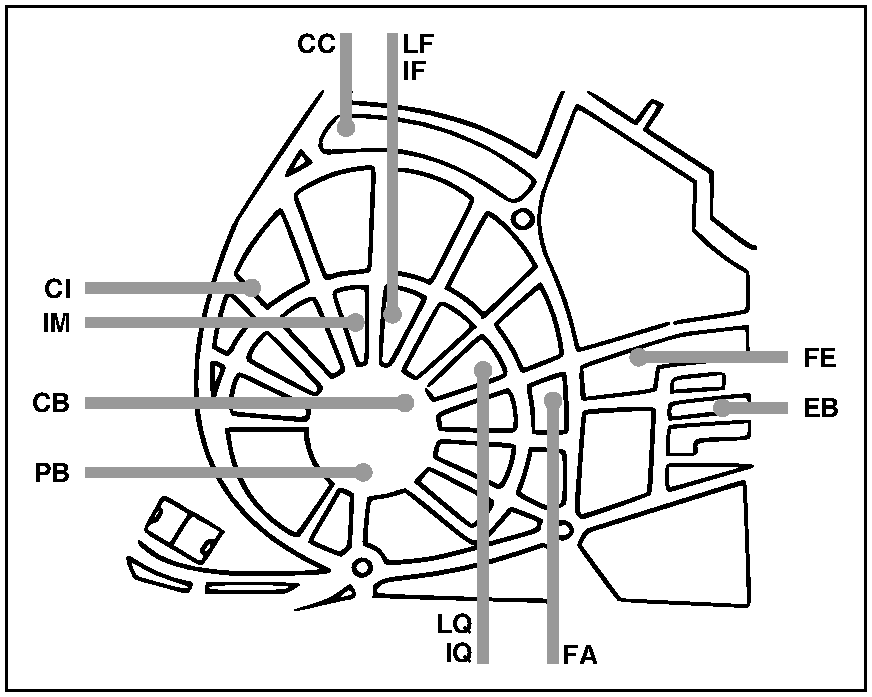
\includegraphics[width=\textwidth]{img/unicamp/mapa_siglas.pdf}
  \caption{Mapa com as siglas da sala de aula}
  \label{fig:mapa_siglas}
\end{figure*}

\subsubsection{SAE (Serviço de Apoio ao Estudante):} É encarregado da execução
de programas de assistência desenvolvidas pela Universidade, por iniciativa
própria ou mediante convênios firmados com entidades especializadas.

\subsubsection{Crédito:} Unidade elementar de horas-aula de qualquer curso da
Unicamp. Um crédito equivale a uma hora-aula semanal, ou a 15 horas-aula
semestrais.

\subsubsection{Período letivo:} É um nome complicado para se referir ao
semestre.

\subsubsection{Currículo pleno:} É o conjunto de disciplinas do curso que o
aluno tem que cursar.

\subsubsection{CR (Coeficiente de Rendimento):} Valor entre 0 e 1 que é a média
das notas obtidas em todas as disciplinas até o momento ponderada pelos
créditos, então ir mal numa matéria de 6 créditos pode prejudicar muito seu CR.

\subsubsection{CP (Coeficiente de Progressão):} É a porcentagem do curso que
você já cumpriu. Por exemplo, se você tem CP = 0,6123 significa que você
cumpriu 61,23\% do curso. Você se forma quando o seu CP for 1 (100\% do curso
completo). É importante saber o CP quando for fazer algum estágio, ou um TCC
(Trabalho de Conclusão de Curso), ou quando for cursar disciplinas que tenham
como pré-requisito AA4xy.

\subsubsection{CPF (Coeficiente de Progressão Futuro):} Além do CP, também tem
o CPF, que além do nome de um documento é o CP que você terá no fim do semestre
caso passe em todas as disciplinas.

\subsubsection{CPE (Coeficiente de Progressão Exigido):} Além do CP e do CPF há
o CPE. O CPE foi instituído a partir de 2005 e é usado para fins de
cancelamento, ou não, de matrícula. Para que o aluno possa continuar a fazer o
curso, ele precisa ter um CP maior ou igual ao CPE daquele semestre. Tanto o
CP, como o CPE e o CPF existem somente nos cursos de graduação.

\subsubsection{Pré-requisito:} Matéria(s) que precisa(m) ter sido cursada(s)
para que se possa fazer outra(s) matéria(s). Existem dois tipos de
pré-requisitos: Os pré-requsitos totais, mais comuns, do qual é exigido tanto a
aprovação por nota como por frequência e os pré-requisitos parciais, mais
raros, do qual o aluno não precisa ter sido aprovado por nota, mas tem que ter
tido aprovação por frequência e nota final maior ou igual a 3,0. Os
pré-requisitos parciais são identificados com um asterisco na frente do código
da disciplina (não confundir com um apontador, uma ferramenta com a qual você
logo irá entrar em contato).

\subsubsection{AA4xy:} Um tipo de pré-requisito. Não se trata de nenhuma
disciplina. Para fazer disciplinas com esse pré-requisito, o aluno tem que tem
um CP maior ou igual a 0,xy.

\subsubsection{AA200:} Outro tipo de pré-requisito existente, mais presente em
disciplinas eletivas. Também não se trata de nenhuma disciplina. É apenas uma
autorização da coordenadoria do curso. Se sobrar vagas para a disciplina e a
coordenadoria do curso for com a sua cara você faz a disciplina.

\subsubsection{PB (Prédio Básico)} Também conhecido como Ciclo Básico II, é um
prédio com várias salas de aula, que fica em frente ao Bandejão, e serve várias
unidades que não possuem espaço físico suficiente para comportar seus alunos.
No segundo andar ficam as salas de aula (PB01 a PB12) e no terceiro andar ficam
os auditórios (PB13 a PB18).

\subsubsection{CB (Ciclo Básico I):} Tem finalidade idêntica ao PB, só que é
muito melhor equipado, tem uma acústica muito melhor e tem um ar condicionado
capaz de matar esquimó de frio. Fica na mesma praça que o PB, só que no outro
extremo. À esquerda da entrada pela rua ficam as salas ímpares e à direita
ficam as salas pares. No primeiro andar ficam os auditórios (CB01 a CB06) que
possuem 140 e 160 lugares e no segundo andar ficam as salas de aula (CB07 a
CB18) que possuem 60 e 80 lugares.  O CB e o PB são os lugares onde você vai
ter a maioria das suas aulas (especialmente nos dois primeiros anos de curso,
então não tem porque procurar morar perto do IC ou da FEEC, cuidado!).

\subsection{Siglas de salas de aula}

A Tabela~\ref{tab:institutos} contém algumas siglas de salas de aula que
aparecem nos cadernos de horários, disponibilizados pelas coordenadorias dos
cursos e pela DAC. E a Figura~\ref{fig:mapa_siglas} aponta a localização das
salas de aula pelas siglas.

\begin{table*}[ht!]
    \centering
    \begin{tabular}{|c|p{.4\textwidth}|p{.45\textwidth}|}\hline
        \multicolumn{3}{|c|}{ \textbf{Siglas e locais das Salas de Aula no
        horário}}\\ \hline

        \textbf{Sigla}  &  \textbf{Local}  &  \textbf{Referência}\\ \hline

        CB  &  Ciclo Básico I  &  Praça Central, atrás do Santander, em frente
        à Cantina da Física.\\ \hline

        CC  &  Instituto de Computação (IC)  &  Ao lado do Departamento de
        Artes Cênicas (IC-1); ao lado do IE (IC-2) e atrás do IE (IC-3).\\
        \hline

        CI  &  Centro de Estudo de Línguas (CEL)  &  Atrás do IFCH.\\ \hline

        CL  &  Instituto de Estudos da Linguagem (IEL)  &  Em frente a praça
        central e ao lado do IFCH.\\ \hline

        EB  &  Engenharia Básica  &  Atrás da Praça da Paz e próximo à FEEC.\\
        \hline

        EM  &  Faculdade de Engenharia Mecânica (FEM)  &  Atrás do IQ.\\ \hline

        FA  &  Faculdade de Engenharia de Alimentos (FEA)  &  Em frente ao IQ
        e à Praça da Paz.\\ \hline

        FE  &  Faculdade de Engenharia Elétrica e de Computação (FEEC)  &  Em
        frente à Praça da Paz.\\ \hline

        IB  &  Instituto de Biologia (IB)  &  Entre o IQ e o Serviço Social do
        SAE.\\ \hline

        IE  &  Instituto de Economia (IE)  &  Atrás do IMECC.\\ \hline

        IF  &  Instituto de Física (IFGW)  &  Em frente ao Ciclo Básico, e a
        Química.\\ \hline

        IH  &  Instituto de Filosofia e Ciências Humanas (IFCH)  &  Entre o
        IMECC e o IEL.\\ \hline

        IM  &  Instituto de Matemática, Estatística e Computação Científica
        (IMECC)  &  Em frente a Praça Central.\\ \hline

        IQ  &  Instituto de Química (IQ)  &  Entre o IB e o IFGW.\\ \hline

        LE  &  Laboratórios de informática da FEEC  &  Em frente a Praça da Paz
        e ao lado das salas de aula da FEEC.\\ \hline

        LF  &  Laboratório de Física  &  Em frente à cantina do IMECC.\\ \hline

        LQ  &  Laboratório de Química  &  Em frente à biblioteca do IQ.\\
        \hline

        PB  &  Ciclo Básico II, Prédio Básico  &  Praça Central, em frente ao
        Bandejão.\\ \hline
    \end{tabular}
    \caption{Siglas das salas de aula}
    \label{tab:institutos}
\end{table*}
